\subsection {Domain Analysis}
\subsubsection{Glossary}
\begin{description}
\item [{Toll~tag}] A toll tag is a physical device which will admit passage
through an express lane when equipped on a vehicle. Toll tags need
to be ordered by customers, and can only be used by one vehicle. The
toll system automatically computes the fare of the vehicle based on
the distance travelled between check in and check out.

\item [{Single~ticket}] Single tickets can be purchased in a cash or credit
card lane, and are valid for 24 hours.

\item [{Toll~Station}] A toll station is a collection of toll lanes. A
station manager is connected to every toll station and can view \emph{statistical
reports}, as well as view and modify customer data.

\item [{Statistical~Report}] Each toll station records which vehicles
purchased single tickets and used toll tags, along with the type of
the vehicle. A statistical report is a writeout of this information
for a given time period.

\item [{Express~Lane}] An express lane will automatically admit passage
to vehicles equipped with a toll tag. The vehicle will be registered
as having passed through the lane at the given time.

\item [{Credit~Card~Lane}] In a credit card lane, the user can use their
credit card to purchase a single ticket.

\item [{Cash~Lane}] A cash lane is manned by a cashier, who accepts cash
payments as well as credit cards. When a cashier mans a credit card
lane, it becomes a cash lane.

\item [{Cashier}] A cashier operates a cash lane and accepts cash payment
in exchange for single tickets.

\item [{Customer}]~

\item [{Rate}]~

\item [{Administrative~Operations}]~
\end{description}


\subsubsection{Domain Model}
\begin{figure}
\centering
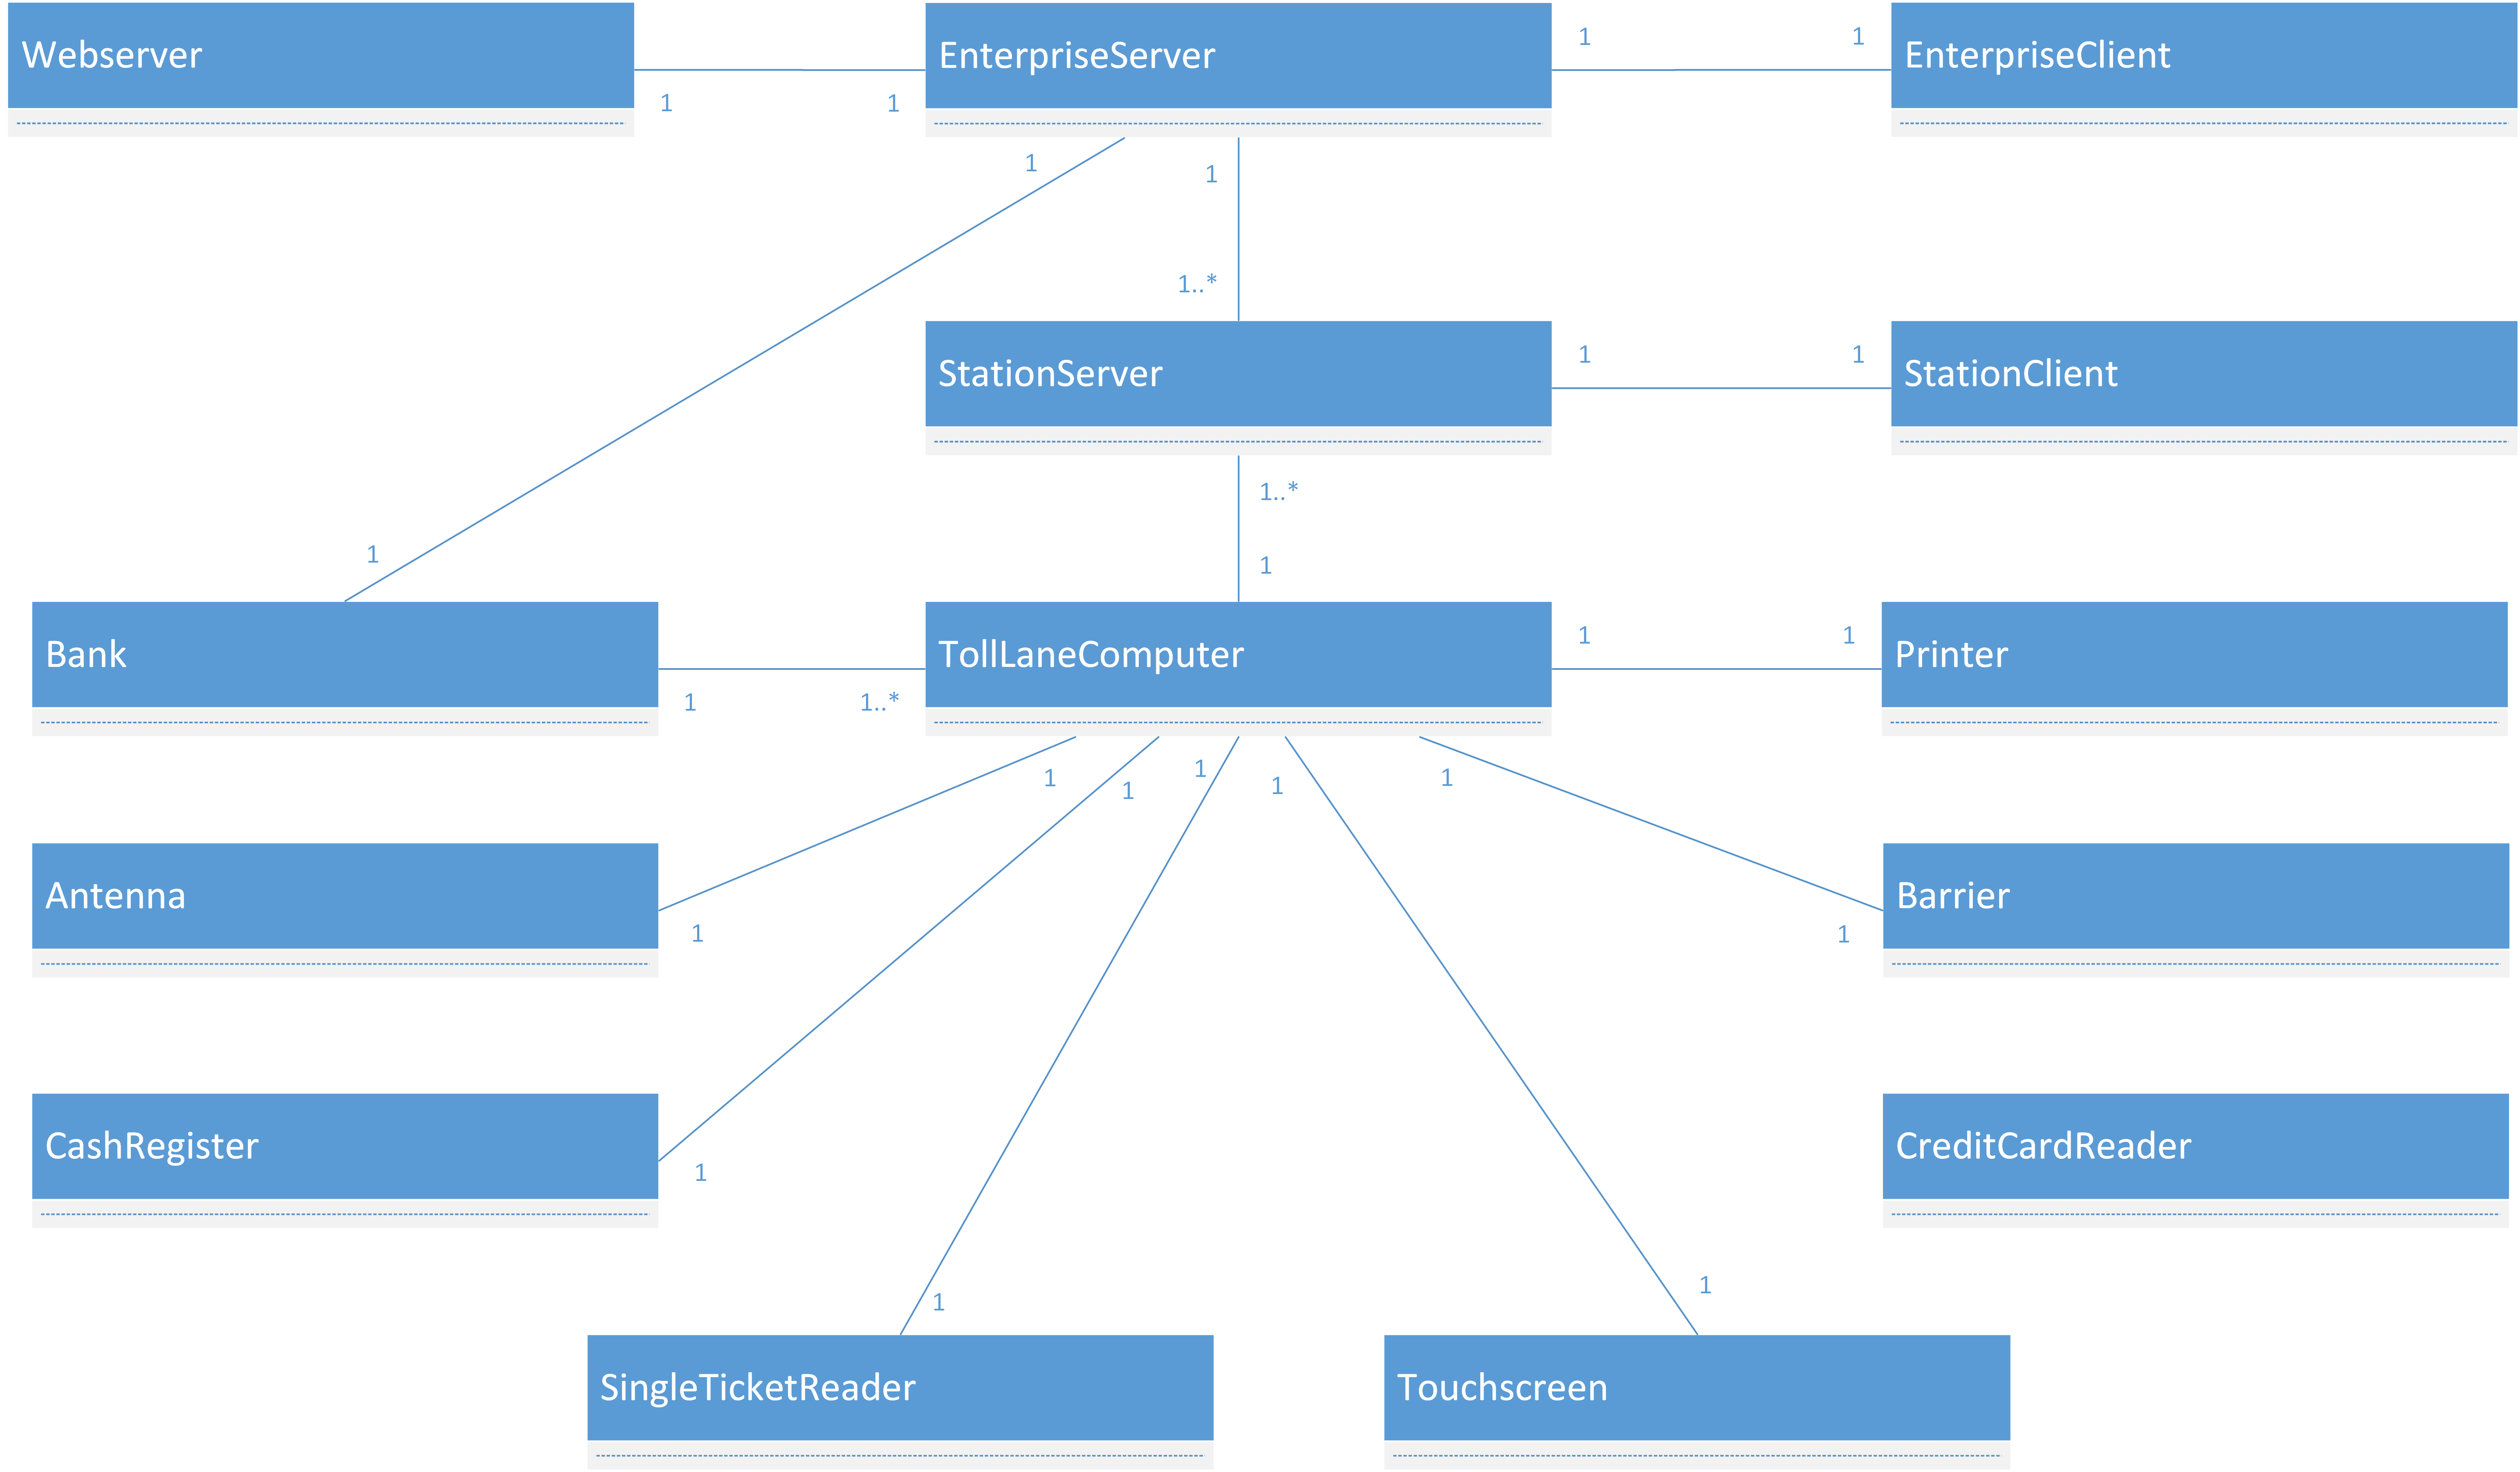
\includegraphics[width=1\textwidth]{img/domain_model/domain_model.png}
\caption{The class diagram depicting the domain model}
\label{fig:domain_model}
\end{figure}

In our domain model in {\autoref{fig:domain_model}}, we have a computer at each toll lane that controls all the components that are part of that lane. All these lane computers are then connected to a station server which controls what goes on at the station. All of the stations for the entire system are then connected to a single enterprise server which manages communication between the stations. For sale of tickets and toll tags our lanes and enterprise server is able to communicate with the bank in order to process those sales.

\begin{description}
\item [{Toll~tag}] A toll tag is a physical device which will admit passage
through an express lane when equipped on a vehicle. Toll tags need
to be ordered by customers, and can only be used by one vehicle. The
toll system automatically computes the fare of the vehicle based on
the distance traveled between check in and check out.


\item [{Toll~Station}] A toll station is a collection of toll lanes. A
station manager is connected to every toll station and can view \emph{statistical
reports}, as well as view and modify customer data.

\item [{Statistical~Report}] Each toll station records which vehicles
purchased single tickets and used toll tags, along with the type of
the vehicle. A statistical report is a write-out of this information
for a given time period.

\item [{Express~Lane}] An express lane will automatically admit passage
to vehicles equipped with a toll tag. The vehicle will be registered
as having passed through the lane at the given time.

\item [{Credit~Card~Lane}] In a credit card lane, the user can use their
credit card to purchase a single ticket.

\item [{Cash~Lane}] A cash lane is manned by a cashier, who accepts cash
payments as well as credit cards. When a cashier mans a credit card
lane, it becomes a cash lane.

\item [{Normal Lane}] A normal lane is an umbrella term for non-express lanes.

\item [{Cashier}] A cashier operates a cash lane and accepts cash payment
in exchange for single tickets.

\item [{Customer}] The customer is the driver of a vehicle.

\item [{Rate}] The price to pay for a certain vehicle type for certain ticket/tag type.

\item [{Enterprise}] The company which control these sections of the motorway.

\item [{Enterprise manager}] The manager who is in charge of all the toll stations.

\end{description}

\subsubsection {Use Case Diagram}

\subsection{Functional Requirements}

\subsubsection{Activity Diagram}

\subsubsection{Detailed Use Case}

\textit {Name: } Buy toll tag

\textit {Description: } A customer orders a toll tag by using the web interface, possibly from a toll station.

\textit {Actors: } A customer.

\textit {Preconditions: } The customer has access to the web interface.

\textit{Main Scenario: }

\begin{enumerate}
	\item The customer fills out the form with their personal, vehicle, and bank information.
	\item The customer submits the form.
\end{enumerate}

\textit{Alternative scenarios: }

\begin{enumerate}
	\item Bank rejects the bank information:
	\begin{enumerate}
		\item Begin the main scenario anew.
	\end{enumerate}
\end{enumerate}

\textit {Name: } Check in single ticket

\textit {Description: } A customer in a vehicle enters the toll lane and buys a single ticket.

\textit {Actors: } A customer and a cashier.

\textit {Preconditions: }  The customer is in a cash lane.

\textit{Main Scenario: }

\begin{enumerate}
	\item The cashier selects the customer's vehicle type.
	\item The system displays the price for the vehicle.
	\item The cashier puts cash in cash register
	\item The system prints the ticket.
	\item The system opens the barrier.
	\item The customer leaves the toll lane.
	\item The system closes the barrier.
\end{enumerate}

\textit{Alternative Scenarios: }
\begin{enumerate}
	\item The cashier is not present, the cash payment fails, or the customer wants to pay with their credit card.
		\begin{enumerate}
			\item The customer selects his vehicle type
			\item The system presents the price for a single ticket.
			\item The customer pays using the card reader.
			\item The system processes the payment successfully.
			\item The system prints the ticket.
			\item The system opens the barrier.
			\item The customer leaves the toll lane.
			\item The system closes the barrier.
		\end{enumerate}
		
	\item The credit card payment does not succeed. 
		\begin{enumerate}
			\item Restart the scenario.
		\end{enumerate}

 \end{enumerate} 
 
 \textit{Note:} 
 \begin{enumerate}
 \item We assume that the customer hands over the correct amount of money to the cashier, and that the cashier deposits the money.
 \item The cash payment fails if the customer does not have enough money.
 \end{enumerate}


\subsection{Non-Functional Requirements}
Usability requirements:
\begin{enumerate}
\item Customers in a normal lane must be able to pay for a ticket (in a check-in lane) or check out a ticket (in a check-out lane), and thereafter drive through the lane, in at most 2 minutes. If the customer requires help from the cashier then the constraint is relaxed to 5 minutes.
\item Customers must be able to drive through an express lane in at most 15 seconds.
\item Cashiers must be able to use the toll lane computer after 2 hours of training with at most 1 error per hour.
\item Enterprise managers must be able to use the station client after 5 hours of training with at most 1 error per hour.
\end{enumerate}


Performance requirements:
\begin{enumerate}
\item Toll tags must be recognized at express lanes in at most 5 seconds.
\item Each toll lane and toll station computer should have an up time of 99.9\%.
\item The enterprise server should have an up time of 99.99\%.
\item The time for the system to generate reports for a single toll station must not exceed 1 minute.
\item Every other administrative tasks must not exceed 30 seconds of computation time.
\end{enumerate}